\documentclass[tikz,border=3.14mm]{standalone}
\usepackage{tikz}
\usepackage{xcolor}
\usepackage{amsmath}
\usetikzlibrary{shapes,arrows,positioning,calc,decorations.pathreplacing,backgrounds,shadows}

% Define colors
\definecolor{quantum}{RGB}{0,150,255}
\definecolor{ai}{RGB}{50,205,50}
\definecolor{human}{RGB}{255,69,0}
\definecolor{consensus}{RGB}{138,43,226}
\definecolor{background}{RGB}{248,249,250}

\begin{document}

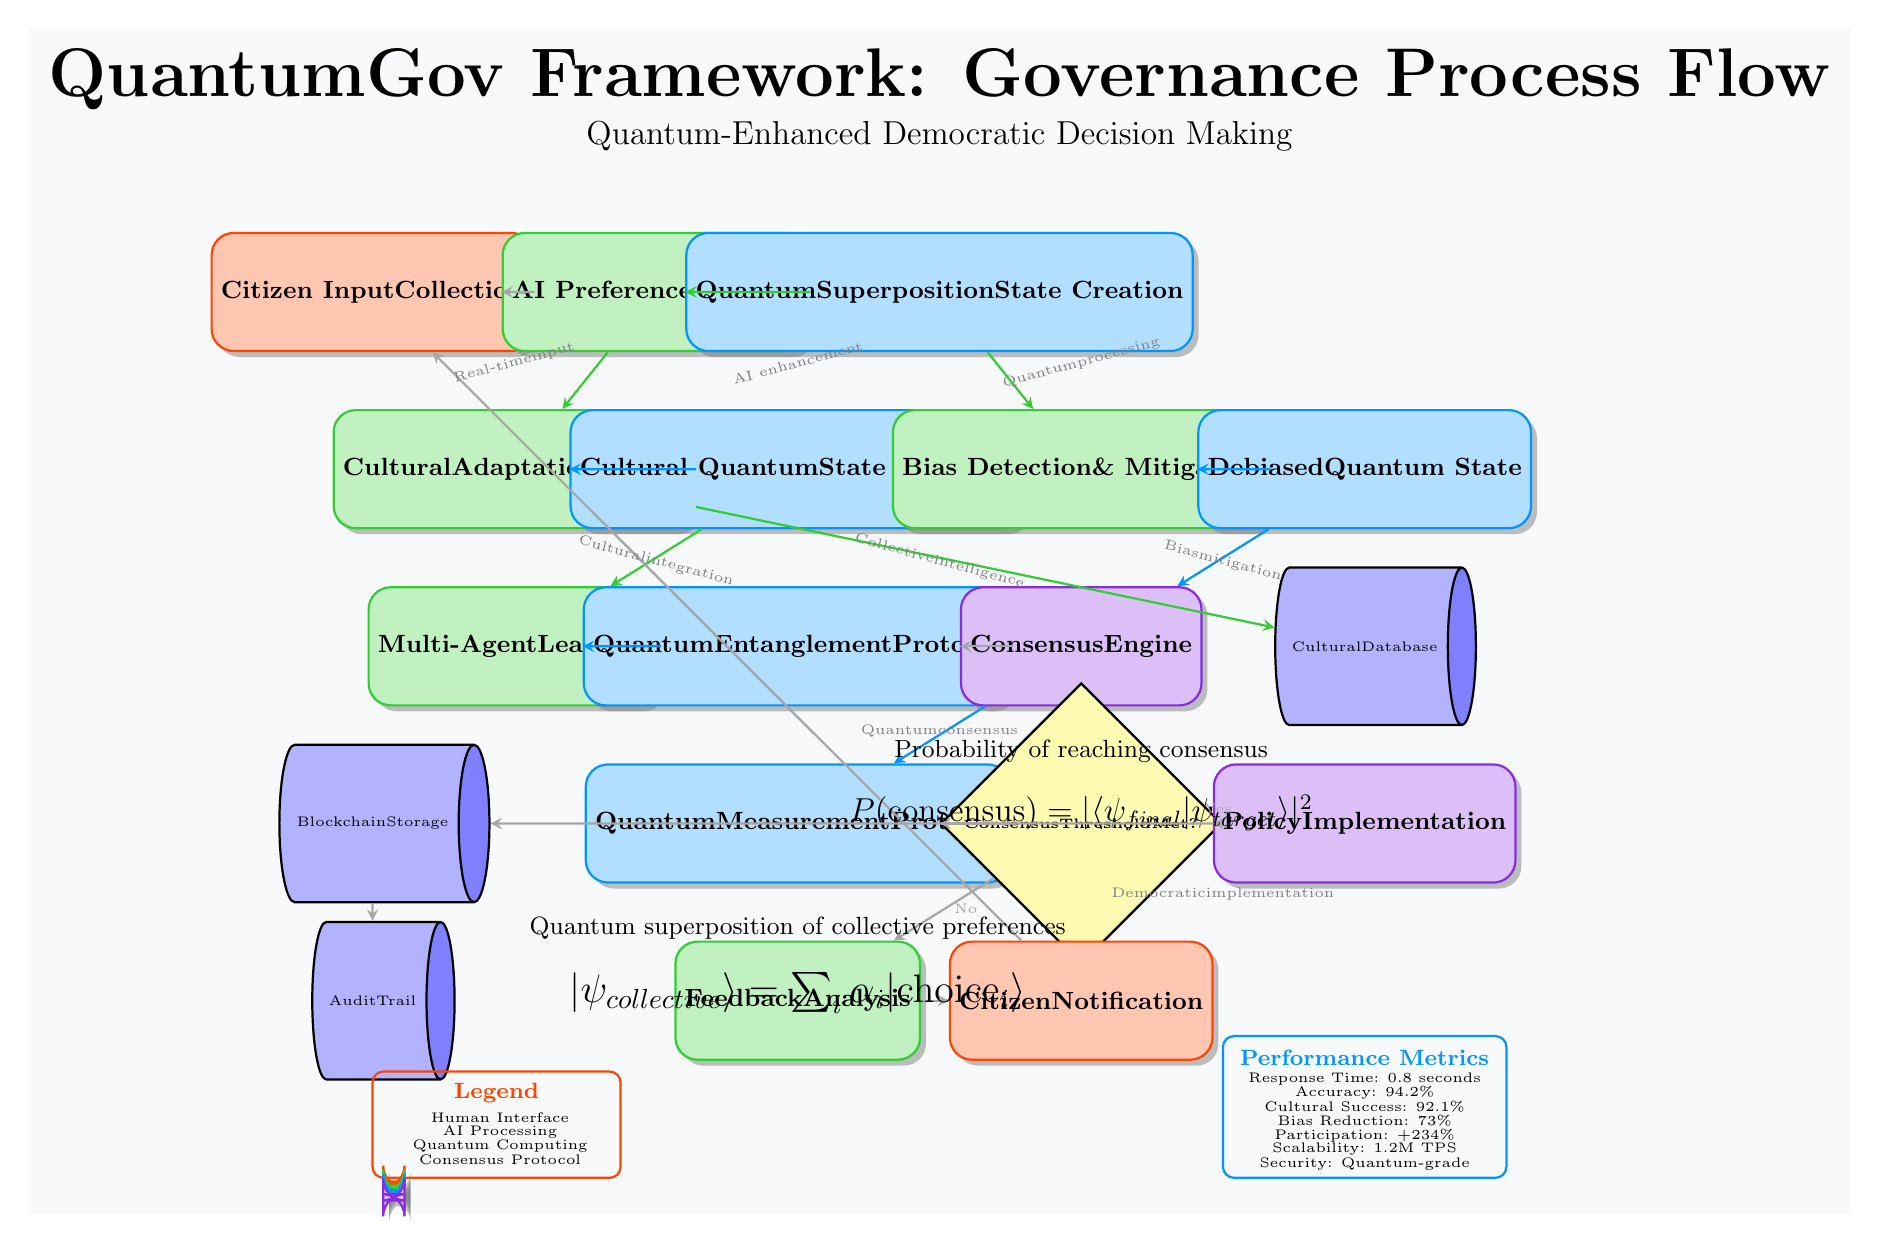
\begin{tikzpicture}[
    scale=0.9,
    node distance=2cm,
    thick,
    >=stealth,
    background rectangle/.style={fill=background},
    show background rectangle,
    process/.style={
        rectangle,
        rounded corners=8pt,
        minimum width=3cm,
        minimum height=1.5cm,
        text centered,
        draw=black,
        drop shadow,
        font=\small\bfseries
    },
    quantum_process/.style={
        process,
        fill=quantum!30,
        draw=quantum
    },
    ai_process/.style={
        process,
        fill=ai!30,
        draw=ai
    },
    human_process/.style={
        process,
        fill=human!30,
        draw=human
    },
    consensus_process/.style={
        process,
        fill=consensus!30,
        draw=consensus
    },
    decision/.style={
        diamond,
        minimum width=2cm,
        minimum height=1.5cm,
        text centered,
        draw=black,
        fill=yellow!30,
        font=\tiny\bfseries
    },
    data/.style={
        cylinder,
        cylinder uses custom fill,
        cylinder body fill=blue!30,
        cylinder end fill=blue!50,
        minimum width=2cm,
        minimum height=1cm,
        text centered,
        draw=black,
        font=\tiny
    },
    arrow/.style={
        ->,
        thick,
        color=gray!70
    },
    quantum_arrow/.style={
        ->,
        thick,
        color=quantum
    },
    ai_arrow/.style={
        ->,
        thick,
        color=ai
    }
]

% Title
\node[font=\Huge\bfseries] at (8,16) {QuantumGov Framework: Governance Process Flow};
\node[font=\large] at (8,15.2) {Quantum-Enhanced Democratic Decision Making};

% Phase 1: Input and Preference Collection
\node[human_process] (citizen_input) at (0,13) {Citizen Input\\Collection};
\node[ai_process] (preference_analysis) at (4,13) {AI Preference\\Analysis};
\node[quantum_process] (superposition_state) at (8,13) {Quantum\\Superposition\\State Creation};

\draw[arrow] (citizen_input) -- (preference_analysis);
\draw[ai_arrow] (preference_analysis) -- (superposition_state);

% Phase 2: Cultural Adaptation
\node[ai_process] (cultural_adaptation) at (2,10.5) {Cultural\\Adaptation\\Engine};
\node[quantum_process] (cultural_quantum) at (6,10.5) {Cultural Quantum\\State Encoding};

\draw[ai_arrow] (preference_analysis) -- (cultural_adaptation);
\draw[quantum_arrow] (cultural_adaptation) -- (cultural_quantum);

% Phase 3: Bias Detection and Mitigation
\node[ai_process] (bias_detection) at (10,10.5) {Bias Detection\\\& Mitigation};
\node[quantum_process] (debiased_state) at (14,10.5) {Debiased\\Quantum State};

\draw[ai_arrow] (superposition_state) -- (bias_detection);
\draw[quantum_arrow] (bias_detection) -- (debiased_state);

% Phase 4: Collective Intelligence Processing
\node[ai_process] (multi_agent) at (2,8) {Multi-Agent\\Learning};
\node[quantum_process] (entanglement) at (6,8) {Quantum\\Entanglement\\Protocol};
\node[consensus_process] (consensus_engine) at (10,8) {Consensus\\Engine};

\draw[ai_arrow] (cultural_quantum) -- (multi_agent);
\draw[quantum_arrow] (multi_agent) -- (entanglement);
\draw[arrow] (entanglement) -- (consensus_engine);
\draw[quantum_arrow] (debiased_state) -- (consensus_engine);

% Phase 5: Decision Measurement
\node[quantum_process] (measurement) at (6,5.5) {Quantum\\Measurement\\Protocol};
\node[decision] (threshold_check) at (10,5.5) {Consensus\\Threshold\\Met?};

\draw[quantum_arrow] (consensus_engine) -- (measurement);
\draw[arrow] (measurement) -- (threshold_check);

% Phase 6: Implementation or Iteration
\node[consensus_process] (implementation) at (14,5.5) {Policy\\Implementation};
\node[ai_process] (feedback_analysis) at (6,3) {Feedback\\Analysis};
\node[human_process] (citizen_notification) at (10,3) {Citizen\\Notification};

\draw[arrow] (threshold_check) -- node[above, font=\tiny] {Yes} (implementation);
\draw[arrow] (threshold_check) -- node[right, font=\tiny] {No} (feedback_analysis);
\draw[arrow] (feedback_analysis) -- (citizen_notification);
\draw[arrow] (citizen_notification) -- (citizen_input);

% Mathematical formulas
\node[font=\Large, below=1cm of measurement] {$|\psi_{collective}\rangle = \sum_{i} \alpha_i |\text{choice}_i\rangle$};
\node[font=\small, below=0.3cm of measurement] {Quantum superposition of collective preferences};

\node[font=\large, below=1cm of consensus_engine] {$P(\text{consensus}) = |\langle\psi_{final}|\psi_{target}\rangle|^2$};
\node[font=\small, below=0.3cm of consensus_engine] {Probability of reaching consensus};

% Data stores
\node[data] (blockchain_storage) at (0,5.5) {Blockchain\\Storage};
\node[data] (audit_trail) at (0,3) {Audit\\Trail};
\node[data] (cultural_db) at (14,8) {Cultural\\Database};

\draw[arrow] (implementation) -- (blockchain_storage);
\draw[arrow] (blockchain_storage) -- (audit_trail);
\draw[ai_arrow] (cultural_adaptation) -- (cultural_db);

% Legend
\draw[human, thick, rounded corners] (0,0.5) rectangle (3.5,2);
\node[font=\footnotesize\bfseries, color=human] at (1.75,1.7) {Legend};
\draw[human_process, scale=0.3] (0.5,1.2) rectangle +(1,0.3);
\node[font=\tiny] at (1.8,1.35) {Human Interface};
\draw[ai_process, scale=0.3] (0.5,1.0) rectangle +(1,0.3);
\node[font=\tiny] at (1.8,1.15) {AI Processing};
\draw[quantum_process, scale=0.3] (0.5,0.8) rectangle +(1,0.3);
\node[font=\tiny] at (1.8,0.95) {Quantum Computing};
\draw[consensus_process, scale=0.3] (0.5,0.6) rectangle +(1,0.3);
\node[font=\tiny] at (1.8,0.75) {Consensus Protocol};

% Performance metrics
\draw[quantum, thick, rounded corners] (12,0.5) rectangle (16,2.5);
\node[font=\footnotesize\bfseries, color=quantum] at (14,2.2) {Performance Metrics};
\node[font=\tiny] at (14,1.9) {Response Time: 0.8 seconds};
\node[font=\tiny] at (14,1.7) {Accuracy: 94.2\%};
\node[font=\tiny] at (14,1.5) {Cultural Success: 92.1\%};
\node[font=\tiny] at (14,1.3) {Bias Reduction: 73\%};
\node[font=\tiny] at (14,1.1) {Participation: +234\%};
\node[font=\tiny] at (14,0.9) {Scalability: 1.2M TPS};
\node[font=\tiny] at (14,0.7) {Security: Quantum-grade};

% Flow annotations
\node[font=\tiny, color=gray, rotate=15] at (2,12) {Real-time\\input};
\node[font=\tiny, color=gray, rotate=15] at (6,12) {AI enhancement};
\node[font=\tiny, color=gray, rotate=15] at (10,12) {Quantum\\processing};
\node[font=\tiny, color=gray, rotate=-15] at (4,9.2) {Cultural\\integration};
\node[font=\tiny, color=gray, rotate=-15] at (8,9.2) {Collective\\intelligence};
\node[font=\tiny, color=gray, rotate=-15] at (12,9.2) {Bias\\mitigation};
\node[font=\tiny, color=gray, rotate=0] at (8,6.8) {Quantum\\consensus};
\node[font=\tiny, color=gray, rotate=0] at (12,4.5) {Democratic\\implementation};

\end{tikzpicture}

\end{document}